\documentclass{udpreport}
\usepackage[utf8]{inputenc}
\usepackage{graphicx}
\usepackage[spanish]{babel}
\usepackage[]{float}

\setlogo{EITFI}


\title{Informe Laboratorio N3}
\author{Cristobal Urra, Alejandro Pacheco, Jonathan Jara\\Profesor: Jaime Alvarez\\Ayudante: Alexis Inzunza}
\date{Abril 2016}

\begin{document}

\maketitle

\tableofcontents
\chapter{Introducción.}
El siguiente informe detalla los pasos realizados por nuestro equipo según lo detallado en el documento .PDF, el trabajo consiste en realizar experimentos con el programa Scapy, encargado de gestionar de diversos modos los paquetes de red, junto al envió de estos mismo haciendo cambios en las direcciones MAC entre otras pruebas detalladas más adelante. Todo analizado y monitoreado por el programa Wireshark.
\chapter{Creación de Paquetes.}
En primer lugar abrimos Scapy 
\begin{figure}[H]
    \centering
    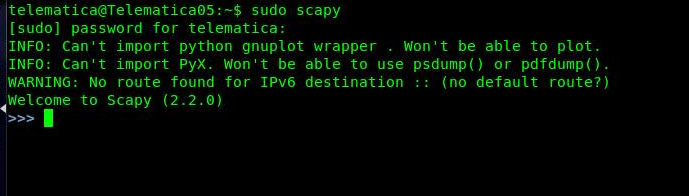
\includegraphics[scale=0.7]{images/ppaso1.png}
    \label{fig:my_label}
\end{figure}

Declaramos la variable Ethernet la cual esta ligada a la funcion Ether()
\begin{figure}[H]
    \centering
    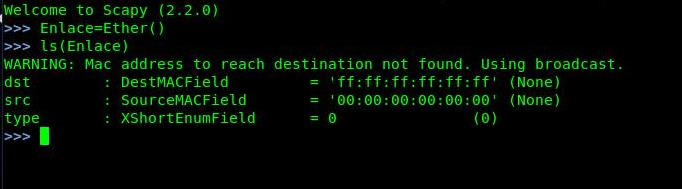
\includegraphics[scale=0.7]{images/ppaso2.png}
    \label{fig:my_label}
\end{figure}
Definimos las direciones MAC con las funciones  Enlace.dst y Enlace.src
\begin{figure}[H]
    \centering
    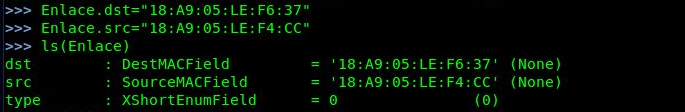
\includegraphics[scale=0.7]{images/ppaso0.png}
    \label{fig:my_label}
\end{figure}
\vspace{14cm}
Declaramos la variable red la cual esta ligada a la funcion IP()
\begin{figure}[H]
    \centering
    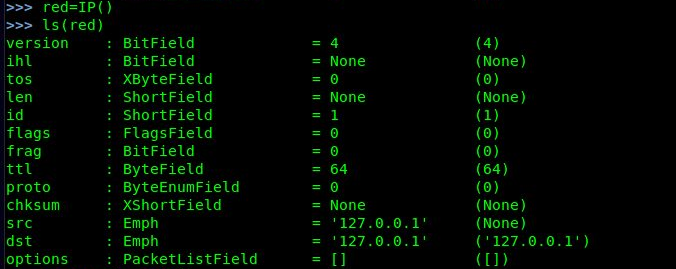
\includegraphics[scale=0.7]{images/ppaso3.png}
    \label{fig:my_label}
\end{figure}
Luego declaramos la variable Transporte la cual esta ligada a la funcion ICMP()
\begin{figure}[H]
    \centering
    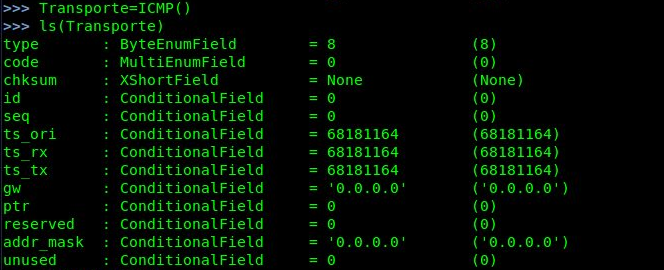
\includegraphics[scale=0.7]{images/ppaso4.png}
    \label{fig:my_label}
\end{figure}
Luego declaramos la variable payload la cual esta ligada a la fucion Raw()
\begin{figure}[H]
    \centering
    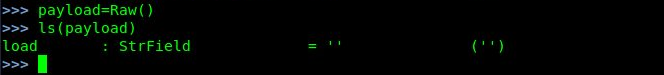
\includegraphics[scale=0.7]{images/ppaso5.png}
    \label{fig:my_label}
\end{figure}
\vspace{14cm}
Luego a la variable paquete la completamos con Enlace/red/Transporte/payload
\begin{figure}[H]
    \centering
    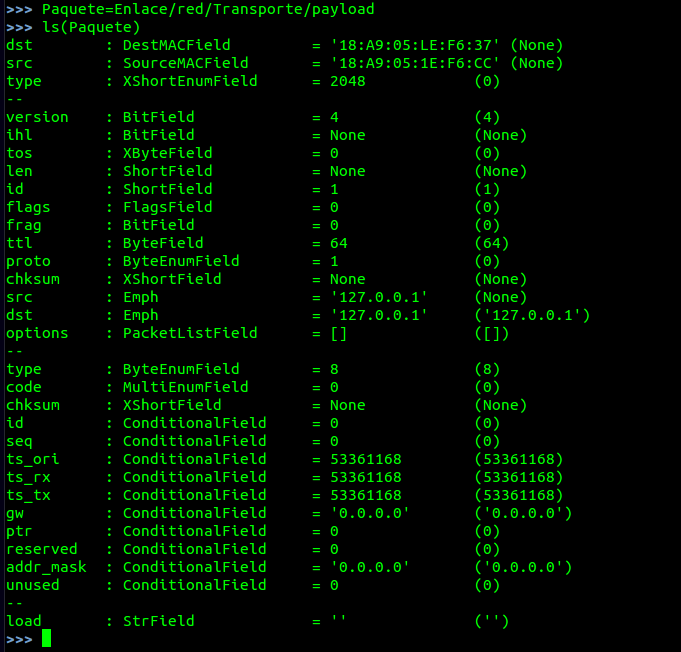
\includegraphics[scale=0.7]{images/ppaso6.png}
    \label{fig:my_label}
\end{figure}
Procedimos a enviarlo con la funcion sendp()
\begin{figure}[H]
    \centering
    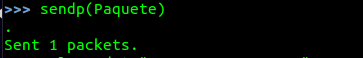
\includegraphics[scale=0.7]{images/ppaso7.png}
    \label{fig:my_label}
\end{figure}
\vspace{14cm}
El paquete llego exitosamente al equipo con la direccion MAC especificada
\begin{figure}[H]
    \centering
    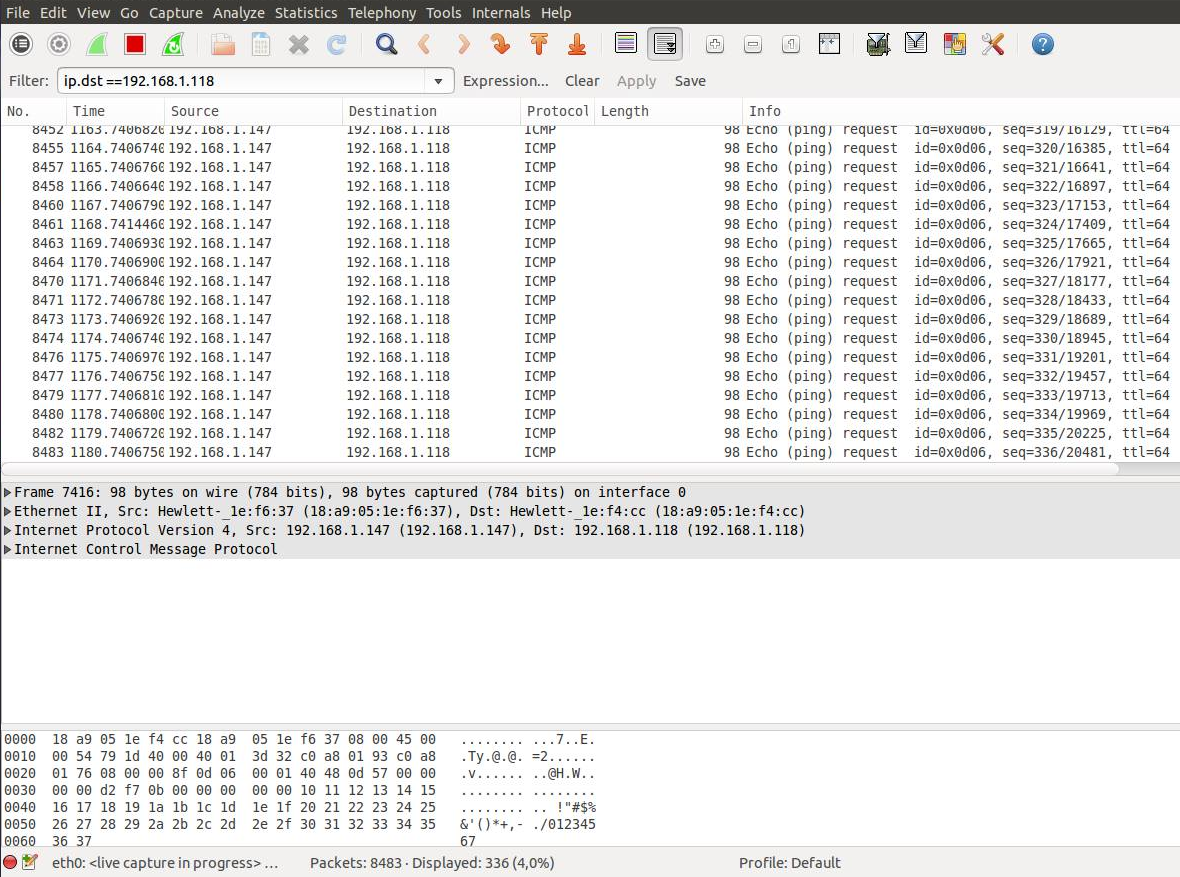
\includegraphics[scale=0.4]{images/wiredef.png}
    \label{fig:my_label}
\end{figure}

\chapter{Cuestionario.}
\section{¿Qué pasa cuando envió un paquete a la dirección\\ FF:FF:FF:FF:FF:FF? ¿Quienes
lo reciben? ¿Por qué?}

El paquete lo recibirán todos los clientes conectados a la red LAN, esto es debido a la MAC especificada como FF:FF:FF:FF:FF es conocida con la dirección MAC de difusión de todas las tarjetas de red en los equipos, en otras palabras es un id universal, el paquete reconocerá esta dirección  en todos lo equipos conectados y por consecuencia todos lo recibirán.

\section{¿Qué pasa cuando envió un paquete a una MAC de otro\\ equipo? ¿Quienes lo
pueden reciben? ¿Por qué?}
El paquete se redirecciona al equipo con la MAC especificada, solo es recibido por este ya que el paquete es de tipo Unicast y el Switch es quien hace el trabajo de enviarlo unicamente a ese equipo, ya que este compara la dirección de destino del paquete y la MAC de los equipos.
\section{¿Qué sucede si envía un paquete a una MAC que no\\ corresponda a ningún equipo
de la red? ¿Quienes lo pueden recepcionar? ¿Por qué?}
El paquete no sería recepcionado por ningún equipo, esto se debe a que al no estar la MAC especificada en la red local, el paquete no sería recibido por ningún equipo capaz de reconocerlo como suyo, los datos se perderían.

\chapter{Conclusion}
Después de analizar los resultados de los experimentos realizados con Scapy y WireShark podemos concluir sobre las vulnerabilidades y los riesgos que se presentan en la gestión y envío de paquetes en una red local, o en casos de enviarlos a una red externa.\\
Las posibilidades de robar paquetes ya sea modificando la dirección MAC o clonando esta misma llaman a el uso de monitoreo y la importancia de la seguridad en las redes.


\end{document}

